\section*{CHƯƠNG 2: LÝ THUYẾT}
\addcontentsline{toc}{section}{\numberline {} CHƯƠNG 2: LÝ THUYẾT}
\setcounter{section}{2}
\setcounter{figure}{0}
\setcounter{subsection}{0}
\subsection{CÔNG NGHỆ LORA}
\subsubsection{Khái niệm}
LoRa là viết tắt của Long Range Radio được nghiên cứu và phát triển bởi Cycleo và sau này được mua lại bởi công ty Semtech năm 2012. Với công nghệ này, chúng ta có thể truyền dữ liệu với khoảng cách lên hàng km mà không cần các mạch khuếch đại công suất; từ đó giúp tiết kiệm năng lượng tiêu thụ khi truyền/nhận dữ liệu. Do đó, LoRa có thể được áp dụng rộng rãi trong các ứng dụng thu thập dữ liệu như sensor network trong đó các sensor node có thể gửi giá trị đo đạc về trung tâm cách xa hàng km và có thể hoạt động với battery trong thời gian dài trước khi cần thay pin.\\
\indent Với tầm xa ,nền tảng không dây công suất thấp là sự lựa chọn công nghệ phổ biến hiện hành để xây dựng mạng iot trên thế giới ứng dụng iot thông minh đã cải thiện theo cách tương tác và giải quết giải quyết một số thách thức lớn nhất mà các thành phố và cộng đồng đang phải đối mặt :biến đổi khí hậu ,kiểm soát ô nhiễm cảnh báo thiên tai và cứu mạng .Kinh doanh cũng được hưởng lợi thông qua cũng như giảm được chi phí. Đây là RF công nghệ không dây được tích hợp vào xe ô tô, đèn đường , sản xuất thiết bị , đồ gia dụng thiết bị đeo được bất cứ điều gì , thực sự . Công nghệ Lora đang làm thế giới ta một hành tinh thông minh\\
\indent Dưới đây là hình ảnh để bạn hiểu rõ nét về tầm xa của Lora:
\begin{figure}[H]
	\centering
	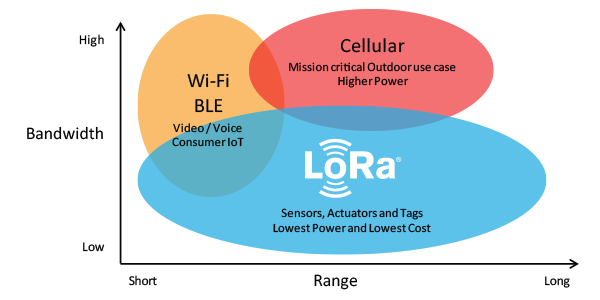
\includegraphics[scale=.5]{Chapter 2/image chapter 2/tamxaLoRa.png}
	\caption[Ảnh minh hoạ tầm xa LoRa]{Ảnh minh hoạ tầm xa LoRa}
	\label{hinh21}
\end{figure}
\subsubsection{Nguyên lý hoạt động}
LoRa sử dụng kỹ thuật điều chế gọi là Chirp Spread Spectrum. Có thể hiểu nôm na nguyên lý này là dữ liệu sẽ được băm bằng các xung cao tần để tạo ra tín hiệu có dãy tần số cao hơn tần số của dữ liệu gốc (cái này gọi là chipped); sau đó tín hiệu cao tần này tiếp tục được mã hoá theo các chuỗi chirp signal (là các tín hiệu hình sin có tần số thay đổi theo thời gian; có 2 loại chirp signal là up-chirp có tần số tăng theo thời gian và down-chirp có tần số giảm theo thời gian; và việc mã hoá theo nguyên tắc bit 1 sẽ sử dụng up-chirp, và bit 0 sẽ sử dụng down-chirp) trước khi truyền ra anten để gửi đi.\\
\indent Theo Semtech công bố thì nguyên lý này giúp giảm độ phức tạp và độ chính xác cần thiết của mạch nhận để có thể giải mã và điều chế lại dữ liệu; hơn nữa LoRa không cần công suất phát lớn mà vẫn có thể truyền xa vì tín hiệu Lora có thể được nhận ở khoảng cách xa ngay cả độ mạnh tín hiệu thấp hơn cả nhiễu môi trường xung quanh.\\
\indent Băng tần làm việc của LoRa từ 430MHz đến 915MHz cho từng khu vực khác nhau trên thế giới:
\begin{itemize}
	\item 430MHz cho châu Á
	\item 780MHz cho Trung Quốc
	\item 433MHz hoặc 866MHz cho châu Âu
	\item 915MHz cho USA
\end{itemize}

\indent Nhờ sử dụng chirp signal mà các tín hiệu LoRa với các chirp rate khác nhau có thể hoạt động trong cùng 1 khu vực mà không gây nhiễu cho nhau. Điều này cho phép nhiều thiết bị LoRa có thể trao đổi dữ liệu trên nhiều kênh đồng thời (mỗi kênh cho 1 chirprate)
\subsubsection{Module thu phát RF UART E32-TTL-100}
\begin{figure}[H]
	\centering
	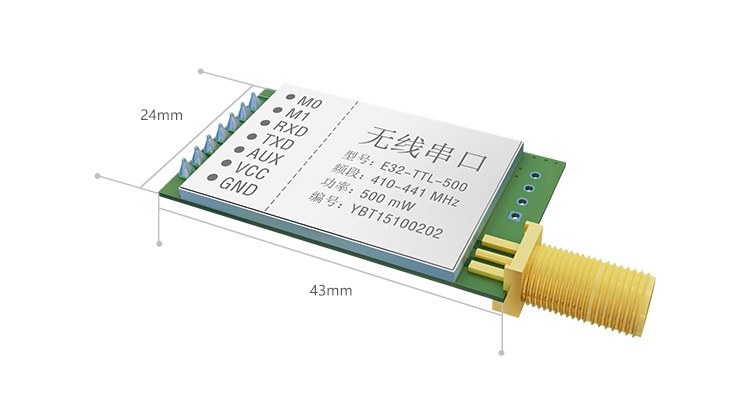
\includegraphics[scale=.4]{Chapter 2/image chapter 2/E32.jpg}
	\caption[Module RF UART E32-TTL-100]{Module RF UART E32-TTL-100}
	\label{hinh22}
\end{figure}
Mạch thu phát RF UART Lora SX1278 433Mhz 3000m sử dụng chip SX1278 của nhà sản xuất SEMTECH chuẩn giao tiếp LORA (Long Range), chuẩn LORA mang đến hai yếu tố quan trọng là tiết kiệm năng lượng và khoảng cách phát siêu xa ( Ultimate long range wireless solution), ngoài ra nó còn có khả năng cấu hình để tạo thành mạng nên hiện tại được phát triển và sử dụng rất nhiều trong các nghiên cứu về IoT.\\
\indent Mạch thu phát RF UART Lora SX1278 433Mhz 3000m được tích hợp phần chuyển đổi giao tiếp SPI của SX1278 sang UART giúp việc giao tiếp và sử dụng rất dễ dàng, chỉ cần kết nối với Software của hãng để cấu hình địa chỉ , tốc độ và công suất truyền là có thể sử dụng.\\
\subsection{GIAO THỨC MQTT}
\subsubsection{Khái niệm}
MQTT (\textbf{Message Queuing Telemetry Transport}) là giao thức truyền thông điệp (message) theo mô hình publish/subscribe (cung cấp /thuê bao), được sử dụng cho các thiết bị IoT với băng thông thấp, độ tin cậy cao và khả năng được sử dụng trong mạng lưới không ổn định. Nó dựa trên một Broker (tạm dịch là “Máy chủ môi giới”) “nhẹ” (khá ít xử lý) và được thiết kế có tính mở (tức là không đặc trưng cho ứng dụng cụ thể nào), đơn giản và dễ cài đặt.\\
\indent MQTT là lựa chọn lý tưởng trong các môi trường như:
\begin{itemize}
	\item Những nơi mà giá mạng viễn thông đắt đỏ hoặc băng thông thấp hay thiếu tin cậy.
	\item Khi chạy trên thiết bị nhúng bị giới hạn về tài nguyên tốc độ và bộ nhớ.
	\item Bởi vì giao thức này sử dụng băng thông thấp trong môi trường có độ trễ cao nên nó là một giao thức lý tưởng cho các ứng dụng M2M (Machine to Machine).
\end{itemize}

\indent MQTT cũng là giao thức được sử dụng trong Facebook Messenger\\
\indent \textbf{Lịch sử hình thành}
\begin{itemize}
	\item MQTT được phát minh bởi Andy Stanford - Clark (IBM) và Arlen Nipper (EUROTECH) cuối năm 1999 khi mà nhiệm vụ của họ là tạo ra một giao thức sao cho sự hao phí năng lượng và băng thông là thấp nhất để kết nối đến đường ống dẫn dầu thông qua sự kết nối của vệ tinh.
	\item Năm 2011, IBM và Eurotech đã trao lại MQTT cho một dự án của Eclipse có tên là Paho.
	\item Năm 2013 MQTT đã được đệ trình lên OASIS (Organization for the Advancement of Structured Information Standards) để chuẩn hóa.
\end{itemize}
\begin{figure}[H]
	\centering
	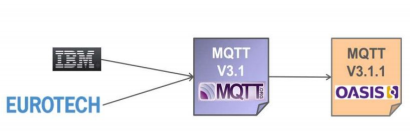
\includegraphics[scale=.7]{Chapter 2/image chapter 2/lichsuMQTT.png}
	\caption[Lịch sử hình thành MQTT]{Lịch sử hình thành MQTT}
	\label{hinh25}
\end{figure}
\subsubsection{Cơ chế hoạt động của MQTT theo mô hình Pub/Sub}
\textbf{Tính chất:}
\begin{itemize}
	\item Space decoupling (Không gian tách biệt).
	\item Time decoupling (Thời gian tách biệt).
	\item Synchronization decoupling (Sự đồng bộ riêng rẽ).
\end{itemize}

\indent \textbf{Đặc điểm riêng:}
\begin{itemize}
	\item MQTT sử dụng cơ chế lọc thông điệp dựa vào tiêu đề (subject-based).
	\item MQTT có một tầng gọi là chất lượng dịch vụ (Quality of Services – QoS). Nó giúp cho dễ dàng nhận biết được là message có được truyền thành công hay không.
\end{itemize}

\indent \textbf{Cơ chế tổng quan}
\begin{figure}[H]
	\centering
	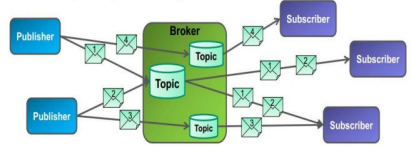
\includegraphics[scale=.7]{Chapter 2/image chapter 2/cochetongquanMQTT.png}
	\caption[Cơ chế tổng quan MQTT]{Cơ chế tổng quan MQTT}
	\label{hinh27}
\end{figure}
MQTT hoạt động theo cơ chế client/server, nơi mà mỗi cảm biến là một khách hàng (client) và kết nối đến một máy chủ, có thể hiểu như một Máy chủ môi giới (broker), thông qua giao thức TCP (Transmission Control Protocol). Broker chịu trách nhiệm điều phối tất cả các thông điệp giữa phía gửi đến đúng phía nhận.\\
\indent MQTT là giao thức định hướng bản tin. Mỗi bản tin là một đoạn rời rạc của tín hiệu và broker không thể nhìn thấy. Mỗi bản tin được publish một địa chỉ, có thể hiểu như một kênh (Topic). Client đăng kí vào một vài kênh để nhận/gửi dữ liệu, gọi là subscribe. Client có thể subscribe vào nhiều kênh. Mỗi client sẽ nhận được dữ liệu khi bất kỳ trạm nào khác gửi dữ liệu vào kênh đã đăng ký. Khi một client gửi một bản tin đến một kênh nào đó gọi là publish.\\
\indent \textbf{Kiến trúc thành phần}
\begin{figure}[H]
	\centering
	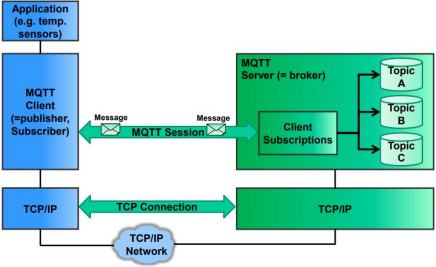
\includegraphics[scale=.7]{Chapter 2/image chapter 2/kientrucMQTT.png}
	\caption[Kiến trúc thành phần MQTT]{Kiến trúc thành phần MQTT}
	\label{hinh28}
\end{figure}
Thành phần chính của MQTT là Client (Publisher/Subscriber), Server (Broker), Sessions (tạm dịch là Phiên làm việc), Subscriptions và Topics.\\
\indent \textit{MQTT Client (Publisher/Subscriber):} Clients sẽ subscribe một hoặc nhiều topics để gửi và nhận thông điệp từ những topic tương ứng.\\
\indent \textit{MQTT Server (Broker):} Broker nhận những thông tin subscribe (Subscriptions) từ client, nhận thông điệp, chuyển những thông điệp đến các Subscriber tương ứng dựa trên Subscriptions từ client.\\
\indent \textit{Topic:} Có thể coi Topic là một hàng đợi các thông điệp, và có sẵn khuôn mẫu dành cho Subscriber hoặc Publisher. Một cách logic thì các topic cho phép Client trao đổi thông tin với những ngữ nghĩa đã được định nghĩa sẵn. Ví dụ: Dữ liệu cảm biến nhiệt độ của một tòa nhà.\\
\indent \textit{Session:} Một session được định nghĩa là kết nối từ client đến server. Tất cả các giao tiếp giữa client và server đều là 1 phần của session.\\
\indent \textit{Subscription:} Không giống như session, subscription về mặt logic là kết nối từ client đến topic. Khi đã subscribe một topic, Client có thể nhận/gửi thông điệp (message) với topic đó.

